\item {\bf Emission Probabilities}

In this problem, we assume that the other car is stationary (e.g., $C_t =
C_{t-1}$ for all time steps $t$). You will implement a function |observe| that
upon observing a new distance measurement $D_t = d_t$ updates the current
posterior probability from
\[\mathbb P(C_t \mid D_1 = d_1, \dots, D_{t-1} = d_{t-1})\]

to
\[\mathbb P(C_t \mid D_1 = d_1, \dots, D_t = d_t) \propto \mathbb P(C_t \mid D_1
= d_1, \dots, D_{t-1} = d_{t-1}) p(d_t \mid c_t),\]

where we have multiplied in the emission probabilities $p(d_t \mid c_t)$
described earlier under ``Modeling car locations". The current posterior
probability is stored as |self.belief| in |ExactInference|.

\begin{center}
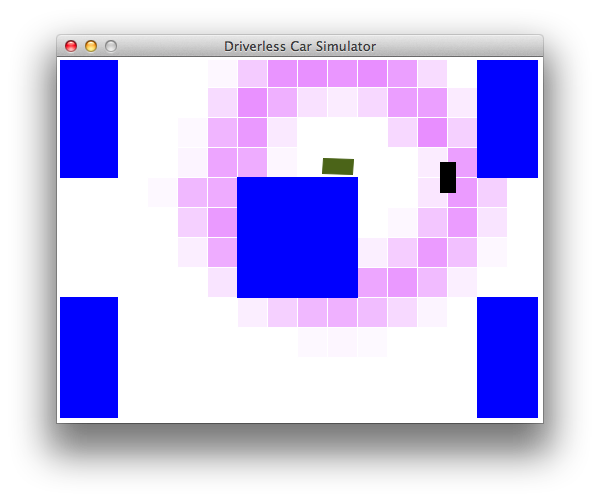
\includegraphics[width=0.5\textwidth]{media/emission.png}
\end{center}

\begin{enumerate}

  \item \points{1a}
Fill in the |observe| method in the |ExactInference| class of |submission.py|.
This method should modify |self.belief| in place to update the posterior
probability of each tile given the observed noisy distance to the other car.
After you're done, you should be able to find the stationary car by driving
around it (using the flag |-p| means cars don't move):

{\em Notes:
\begin{itemize}
  \item You can start driving with exact inference now. 

\begin{lstlisting}
python drive.py -a -p -d -k 1 -i exactInference
\end{lstlisting}
  You can also turn off |-a| to drive manually.

  \item  It's generally best to run |drive.py| on your local machine, but if you
  do decide to run it on remote machine instead, please ssh with either the |-X|
  or |-Y| option in order to get the graphical interface; otherwise, you will get
  some display error message. Note: in this case, expect this graphical interface
  to be a bit slow...

  |drive.py| is not used for grading, but is just there for you to visualize and
  enjoy the game!

  \item Read through the code in util.py for the |Belief| class before you get
  started. You'll need to use this class for several of the code tasks in this
  assignment.

  \item Remember to normalize the posterior probability after you update it.
  (There's a useful function for this in util.py).

  \item On the small map, the autonomous driver will sometimes drive in circles
  around the middle block before heading for the target area. In general, don't
  worry too much about the precise path the car takes. Instead, focus on whether
  your car tracker correctly infers the location of other cars.

  \item Don't worry if your car crashes once in a while! Accidents do happen,
  whether you are human or AI. However, even if there was an accident, your driver
  should have been aware that there was a high probability that another car was in
the area.
\end{itemize}}


\end{enumerate}
